\section{Techniques}

This section gives an overview of different techniques used in our crawler. We first show how we integrated a headless web browser into the harvesting process to support blogs that use JavaScript to display page content. The overall software architecture with then be discussed, introducing the Scrapy framework and the different addition we implemented for our use case.

\subsection{JavaScript rendering}
% Introduction
JavaScript is a widely used use language for client-side web scripting. While some applications simply use it for aesthetics aspects such as menus and animations, an increasing number of websites use JavaScript to download and display content. In such circumstances, traditional HTML based crawled would not see the web site as it would be presented to a human visitor and might therefore be obsolete for extracting data from the page.

% Motivation
In our specific use case of crawling the blog sphere, we encountered several blogs where data was missed because of the lack of JavaScript interpretation. The most frequent cases where blogs using the Disqus\cite{disqus2013} and LiveFyre\cite{livefyre2013} comment hosting services. These tools are very handy to setup for webmasters because the entire comments infrastructure is externalized and the setup essential comes down to including a JavaScript snippet in the target web page. Both of these services heavily rely on JavaScript to download and display the comments, even providing functionalities such as real-time update of comments there are written by users. Less commonly, some blogs are fully rendered using JavaScript. Concretely, when loading such website the web browser will not receive the page content inside an HTML page, but will instead have to execute a script containing the procedure to download and display the page content. On example can be found on the Blogger platforms which proposes as one of its default templates the \emph{Dynamic Views} \cite{antinharasymiv2011} that use this mechanism.

% The solution
To support blogs with JavaScript generated content we embed a full web browser into the crawler. After considering multiple option, we opted for PhantomJS\cite{phantomjs2013}, a headless web browser with great performances and scripting capabilities. In order to take full advantage of all the extraction functionalities, the JavaScript rendering is done as the very first step of blog post processing. This way, every other part of the project is independent of whether or not the page its currently processing was actually rendered by PhantomJS or comes directly from the web server. Extracting blog post content, comments and images therefore works equally well on both blogs with JavaScript generated content and traditional HTML blogs.

% Click click scripting
In addition to extracting page after JavaScript execution, we also use some of PhantomJS scripting capabilities. When the number of comments on one page exceeds a certain threshold, both Disqus and LiveFyre only load a subset of them and end the stream of comments with a \emph{Show More Comments} buttons. As part of the page load process we instruct PhantomJS to repeatedly click on this button until all comments are loaded. As you will see in the evaluation section, \TODO{we will see..}

% \subsection{Architecture}
% \subsubsection{Item pipeline}
% - item pipeline, modularity \\

\subsection{Architecture}

\begin{figure}
  \centering
  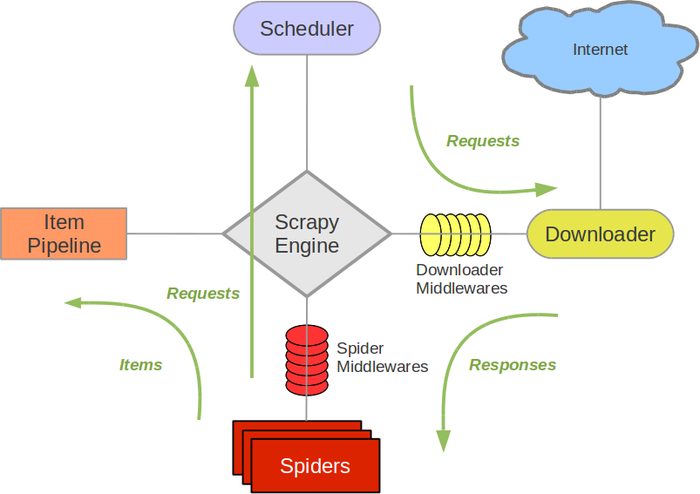
\includegraphics[width=0.47\textwidth]{img/scrapy_architecture.png}
  \caption{Overview of the crawler architecture.}
  \label{architecture}
\end{figure}

Our project is build on top of Scrapy\cite{scrapy2013}, an open source Python framework for web crawling. Scrapy provide an elegant and modulable high-level architecture which we followed in our implementation of the BlogForever Crawler. As illustrated in Figure~\ref{architecture}, Scrapy is divided in several components: \emph{Spiders}, \emph{Item Pipeline}, \emph{Downleader Middlewares} and \emph{Spider Middlewares}, where each of can be used to implement a different functionality.

Our use case has two types of spiders: NewCrawl and UpdateCrawl, which respectively implement the logic to crawl a new blog and to get updates from a previously crawled blog. After downloading the HTML page, blog posts are packed into Items and sent through the folloing pipeline of operation:
\begin{enumerate}[noitemsep]
  \item Render JavaScript
  \item Extract content
  \item Extract comments
  \item Download images
  \item Propagate resulting records to the Invenio backend
\end{enumerate}
This pipeline design, often called the \emph{pipes and filters pattern}\cite[Chapter Messaging Systems]{hohpe2003}, provides great modularity. Indeed, disabeling JavaScript rendering or plugging in an alternative backend can be done by editing a single configuration line.


The default Scrapy behavior
** In addition to the extraction aspects of the project, we also

\subsection{Enriching Scrapy}
In order to find and identify blog posts, our implementation enriches Scrapy with two components to narrow the extraction process to the subsets of blog pages holding blog posts: blog-post identification and download priority heuristic. Given an entry point to a website, the default Scrapy behavior allows to look over all pages of the same domain in a \emph{last in first out} manner. The \emph{blog-post identification} function is able to identify from a URL whether or not the corresponding page is a blog-post. Internally, this function uses a regular expression constructed for each blog from it's web feed entries. These constitute the only set of known blog post URLs, and can therefore be used identify the structure of blog post URLs. This simple approach requieres that blog uses the same pattern for all posts (or false negative will occur) which has to be distinct for non post pages (or false positive will occur) has showed to be .....................................

In order to efficiently deal with blogs with a large number non-blog-post pages, this mechanism is not sufficient. Indeed, after all pages identify as blog-post are processed, the crawler needs to download non-blog-post pages to search for additional blog-posts. To replace the naive random walk, depth first search or breadth first search web site traversals, we use a priority queue where URL priorities are determined by a simple machine learning system. Given an URL, the machine learning system predicts the number of links to blog-post the corresponding page will contain. Each time a page is effectively downloaded, the actual number of blog-post links it contains is computed and given to the machine learning system that will store this value and take it into account for its future prediction. This mechanism has shown to be indispensable for web sites that host on the single domain a blog along with a large number of non-blog web pages, such as a forum or a wiki.

Due to space constraints, more precise description and evaluation of these two components where not included in this paper.


\subsection{Scalability}
Scrapy is written with Twisted, a popular event-driven networking framework for Python. Thus, it’s implemented using a non-blocking (aka asynchronous) code for concurrency.

Scrapy uses the Twisted\cite{twisted2013} asynchronous networking engine

At the time of writing...
- http://www.reactivemanifesto.org/
- stateless \\
- scrapyd \\
